% Propósito: identificar los elementos ideales del modelo
% masa--resorte--amortiguador y las magnitudes asociadas.
% Origen: F_el=-kx, F_amort=-bv y F_ext-kx-bv=ma, ecuaciones
% \eqref{eq:u2-hooke}, \eqref{eq:u2-amortiguamiento} y \eqref{eq:u2-msa}.
% Esquema cualitativo, no a escala.
% Descripción accesible: una masa m puede desplazarse horizontalmente. Está
% conectada en paralelo a una pared mediante un resorte de rigidez k y un
% amortiguador de coeficiente b. Una fuerza externa F_ext apunta hacia el
% sentido positivo del desplazamiento x.
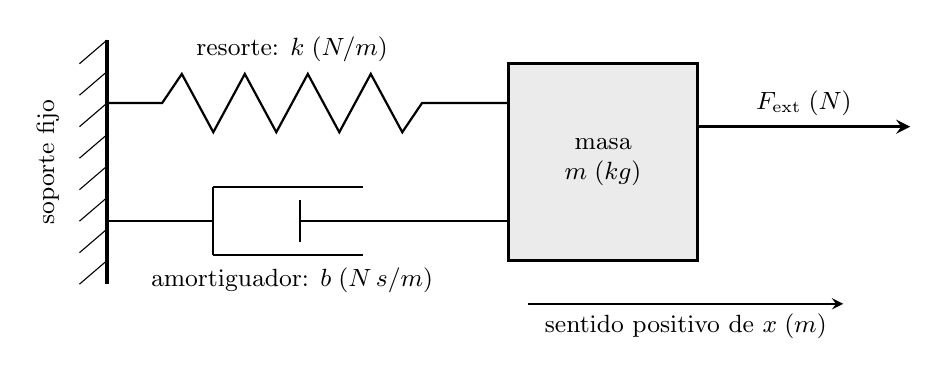
\begin{tikzpicture}[font=\small,>=stealth,x=1cm,y=1cm]
    % Pared fija.
    \draw[very thick] (0,-1.55) -- (0,1.55);
    \foreach \y in {-1.4,-1.0,...,1.4}{
        \draw (-0.35,\y-0.15) -- (0,\y+0.15);
    }
    \node[rotate=90] at (-0.75,0) {soporte fijo};

    % Resorte.
    \draw[thick] (0,0.75) -- (0.7,0.75)
        -- (0.95,1.12) -- (1.35,0.38)
        -- (1.75,1.12) -- (2.15,0.38)
        -- (2.55,1.12) -- (2.95,0.38)
        -- (3.35,1.12) -- (3.75,0.38)
        -- (4.0,0.75) -- (5.1,0.75);
    \node[above] at (2.35,1.15) {resorte: \(k\;(\text{N}/\text{m})\)};

    % Amortiguador viscoso ideal.
    \draw[thick] (0,-0.75) -- (1.35,-0.75);
    \draw[thick] (1.35,-1.18) -- (1.35,-0.32);
    \draw[thick] (1.35,-1.18) -- (3.25,-1.18);
    \draw[thick] (1.35,-0.32) -- (3.25,-0.32);
    \draw[thick] (2.45,-1.02) -- (2.45,-0.48);
    \draw[thick] (2.45,-0.75) -- (5.1,-0.75);
    \node[below] at (2.35,-1.22)
        {amortiguador: \(b\;(\text{N}\,\text{s}/\text{m})\)};

    % Masa y fuerza externa.
    \draw[very thick,fill=black!8] (5.1,-1.25) rectangle (7.5,1.25);
    \node[align=center] at (6.3,0)
        {masa\\\(m\;(\text{kg})\)};
    \draw[->,very thick] (7.5,0.45) -- (10.2,0.45)
        node[midway,above] {\(F_\mathrm{ext}\;(\text{N})\)};
    \draw[->,thick] (5.35,-1.8) -- (9.35,-1.8)
        node[midway,below] {sentido positivo de \(x\;(\text{m})\)};
\end{tikzpicture}
